\chapter{Конструкторский раздел}
\label{cha:design}

В данном разделе приводится описание разработанного метода и его ограничения. Детально рассматриваются применяемые на каждом из этапов алгоритмы.

\section{Статический метод поиска гонок на основе относительного множества блокировок}

Разработанный метод статического поиска гонок в программах на языке Си основан на методе статического поиска гонок Relay \cite{Relay}. В основе метода лежит понятие относительного множества блокировок. Метод состоит из 4 этапов:

\begin{itemize}
  \item построение ГПУ функций,
  \item построение путей выполнения  функций,
  \item построение таблиц защищённого доступа для потоков,
  \item определение мест возможного возникновения гонок.
\end{itemize}

Схема метода представлена на рис.~\ref{fig:idef0-black-box} и на рис.~\ref{fig:idef0}. На вход метода подаётся иходный код программы. Выходом является список мест возможного возникновения гонок. Рассмотрим далее каждый из этапов метода подробнее.

\begin{figure}
  \centering
  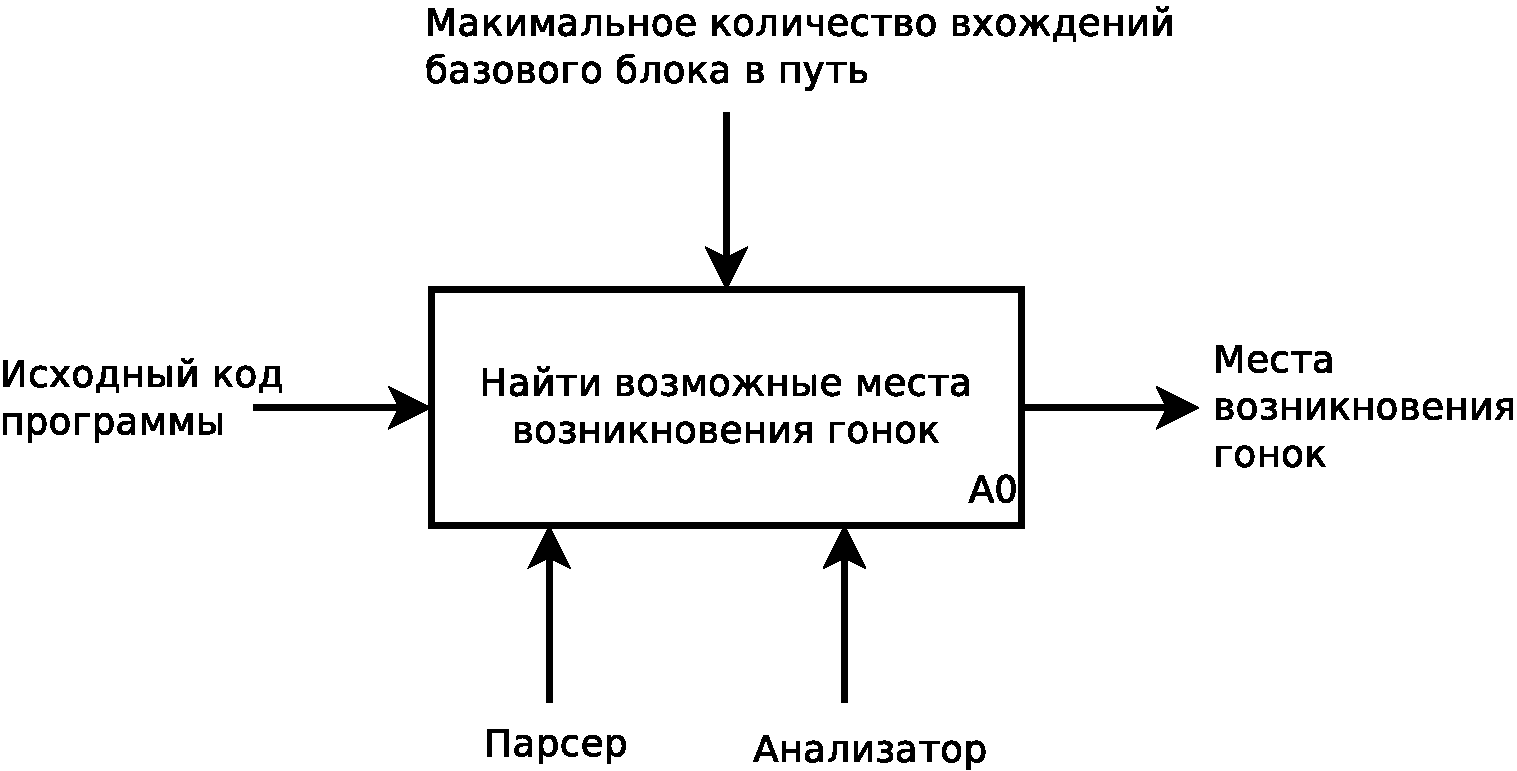
\includegraphics[width=0.6\textwidth]{inc/dia/idef0-black-box}
  \caption{Статический метод поиска гонок на основе относительного множества блокировок}
  \label{fig:idef0-black-box}
\end{figure}

\begin{figure}
  \centering
  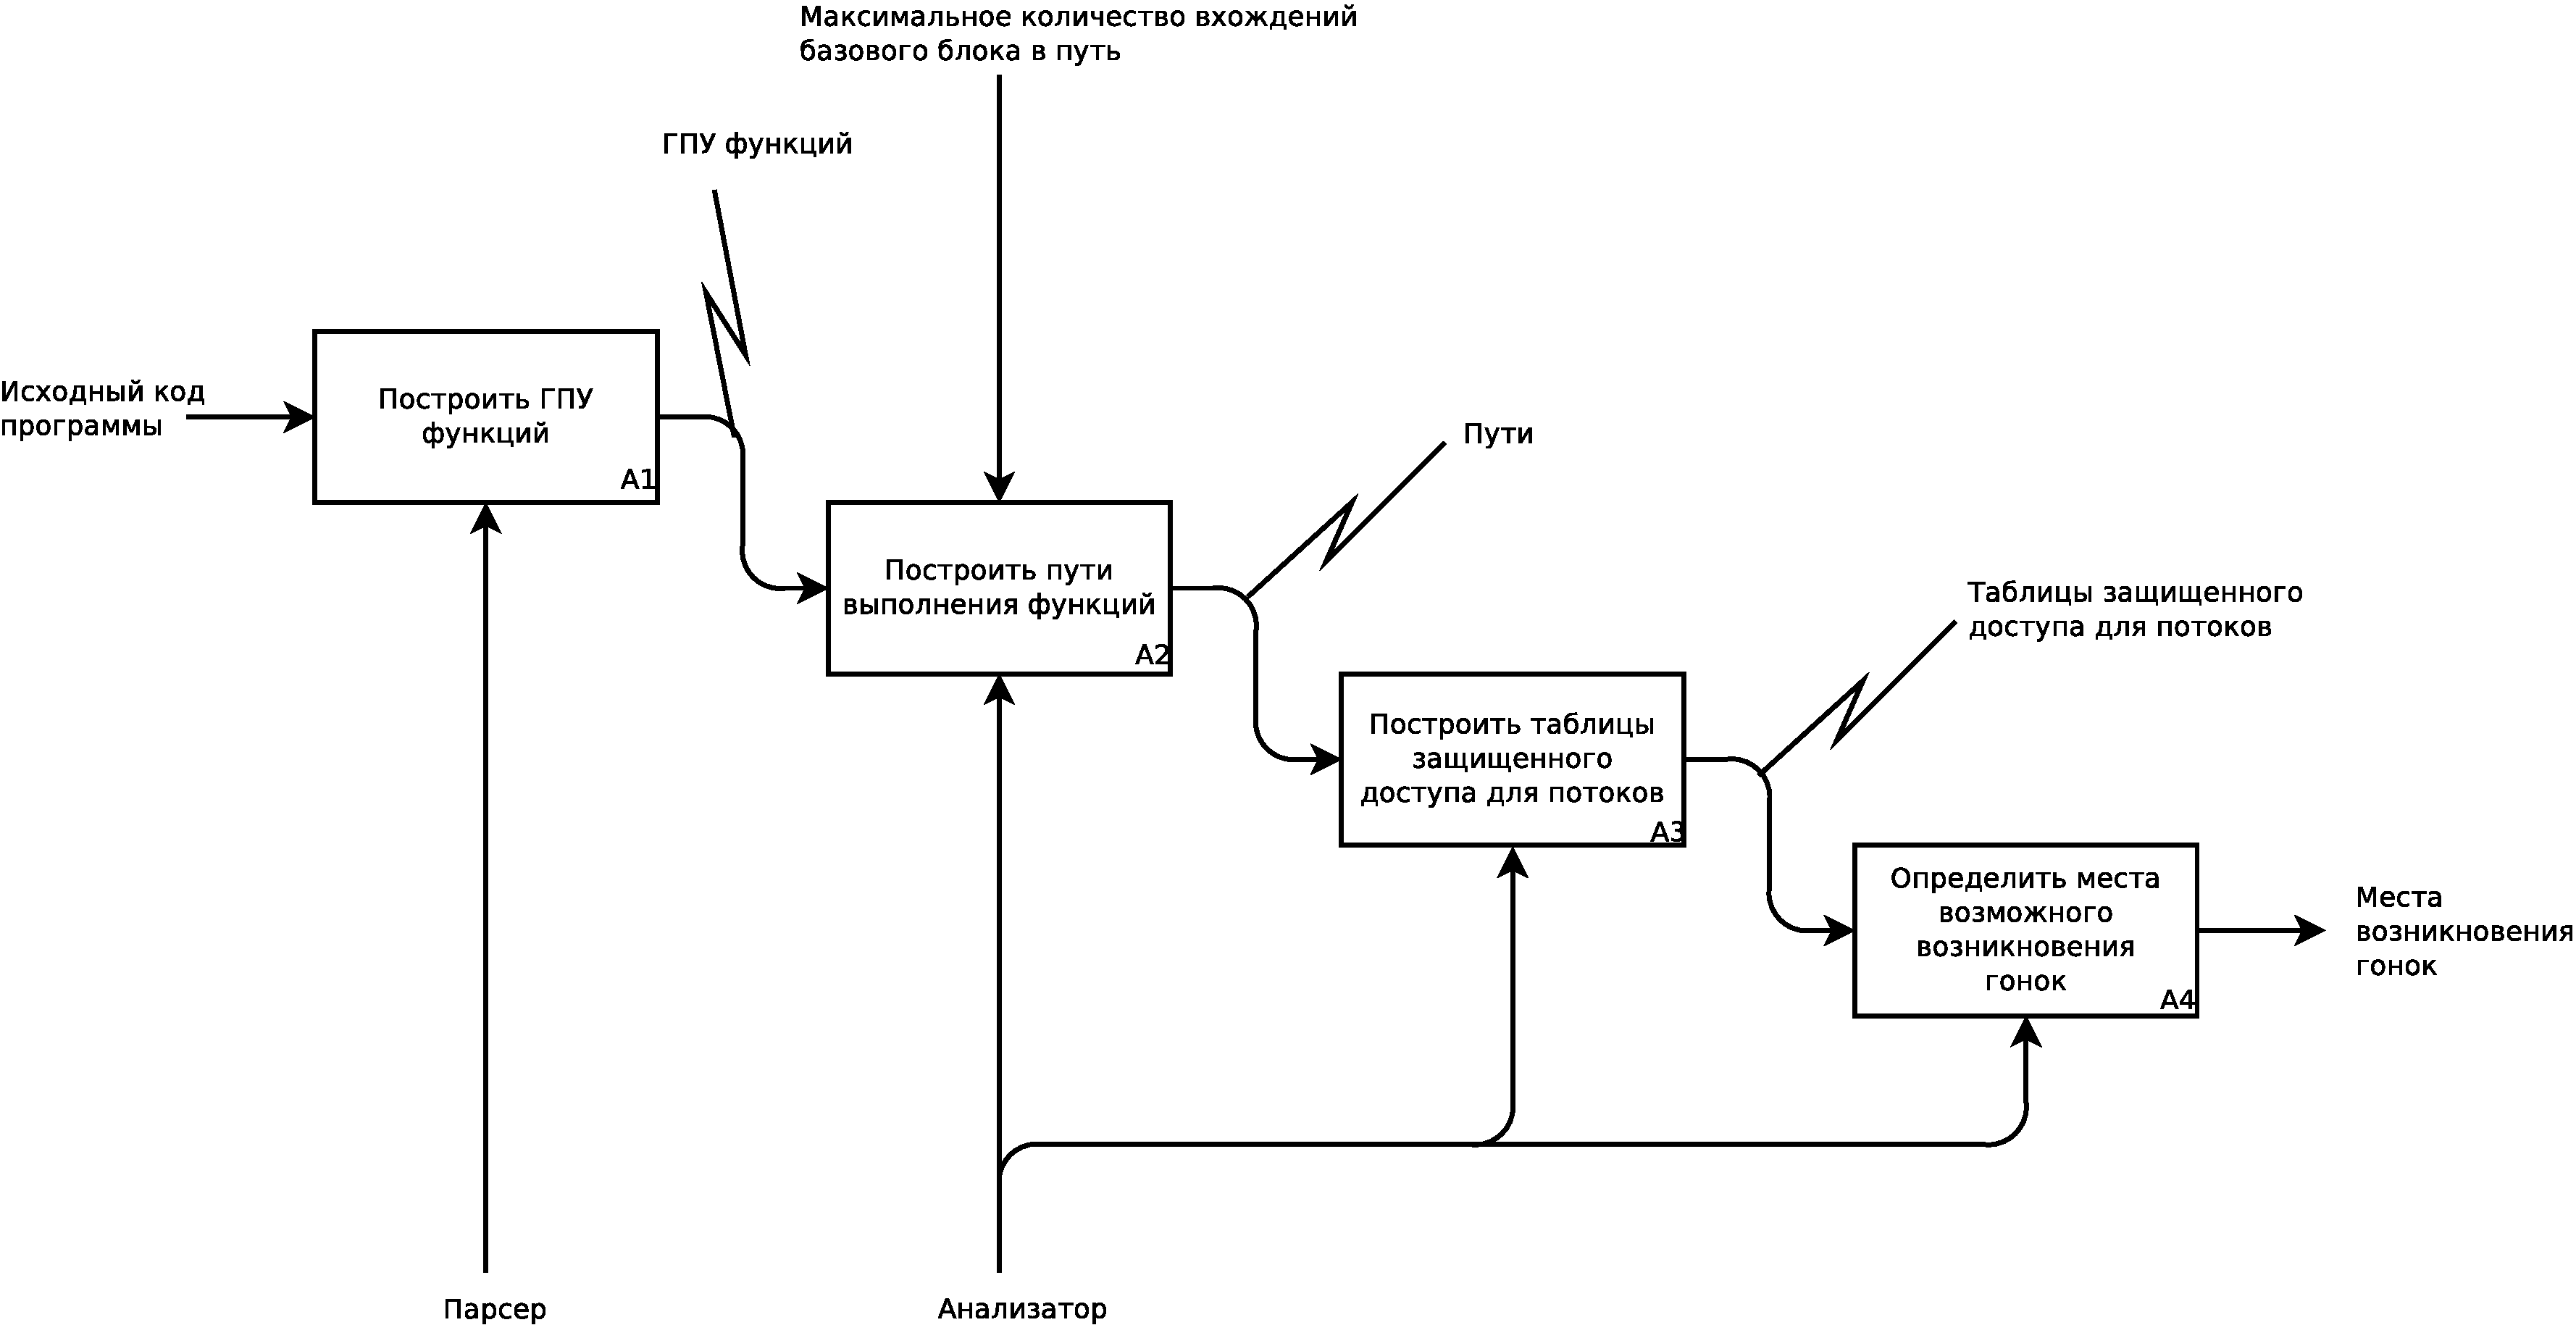
\includegraphics[width=\textwidth]{inc/dia/idef0}
  \caption{Статический метод поиска гонок на основе относительного множества блокировок}
  \label{fig:idef0}
\end{figure}

\section{Ограничения разрабатываемого метода}

К проверяемым программам предъявляются следующие ограничения:
\begin{itemize}
  \item отсутствие рекурсивных вызовов функций,
  \item отсутствие указателей на функции,
  \item отсутствие обращений к памяти по заранее определенным адресам,
  \item отсутствие динамического выделения памяти,
  \item отсутствие арифметики указателей,
  \item отсутствие обращений к элементам массива.
\end{itemize}

%\section{Построение ГПУ функций}
%нужно? (пока убрал)
 
\section{Построение путей выполнения функций}

При построении списка анализируемых путей выполнения функции используется алгоритм, основанный на обходе графа в глубину. Для того, чтобы избежать появления путей бесконечной длины, которые могут появляться в случае наличия циклов в анализируемом графе потока управления, вводится ограничение $K$ на максимальное количество вхождений каждого базового блока в анализируемый путь.

Схема рекурсивного алгоритма обхода графа для построения списка анализируемых путей представлена на рис.~\ref{fig:build-pathes}. При построении путей используется функция \textbf{walk}, которая принимает на вход текущий базовый блок $v$, пройденный путь $p$ и граф потока управления анализируемой функции $G$. Вначале функции \textbf{walk} текущая вершина $v$ добавляется в путь $p$, множество построенных путей $S$ полагается пустым. Затем проверятся является ли вершина $p$ заключительной. Если является, то функция \textbf{walk} возвращает множество построенных путей, включающее в себя только один путь $p$. Иначе - производится рекурсивный запуск функции \textbf{walk} для всех вершин $w$ таких, что существует дуга, началом которой является вершина $v$, а концом - вершина $w$, и вершина $w$ встречается в пути $p$ не более $K$ раз. Возвращаемые при этом  множества включаются в множество $S$. Если вершина $w$ встречается в пути более $K$ раз, то к пути $p$ добавляется заключительная вершина графа потока управления анализируемой функции, и полученный путь добавляется также к $S$. Для получения множества анализируемых путей функции необходимо подать на вход функции \textbf{walk} начальную вершину графа потока управления функции, пустой путь и непосредственно сам анализируемый граф потока управления функции.

\begin{figure}
  \centering
  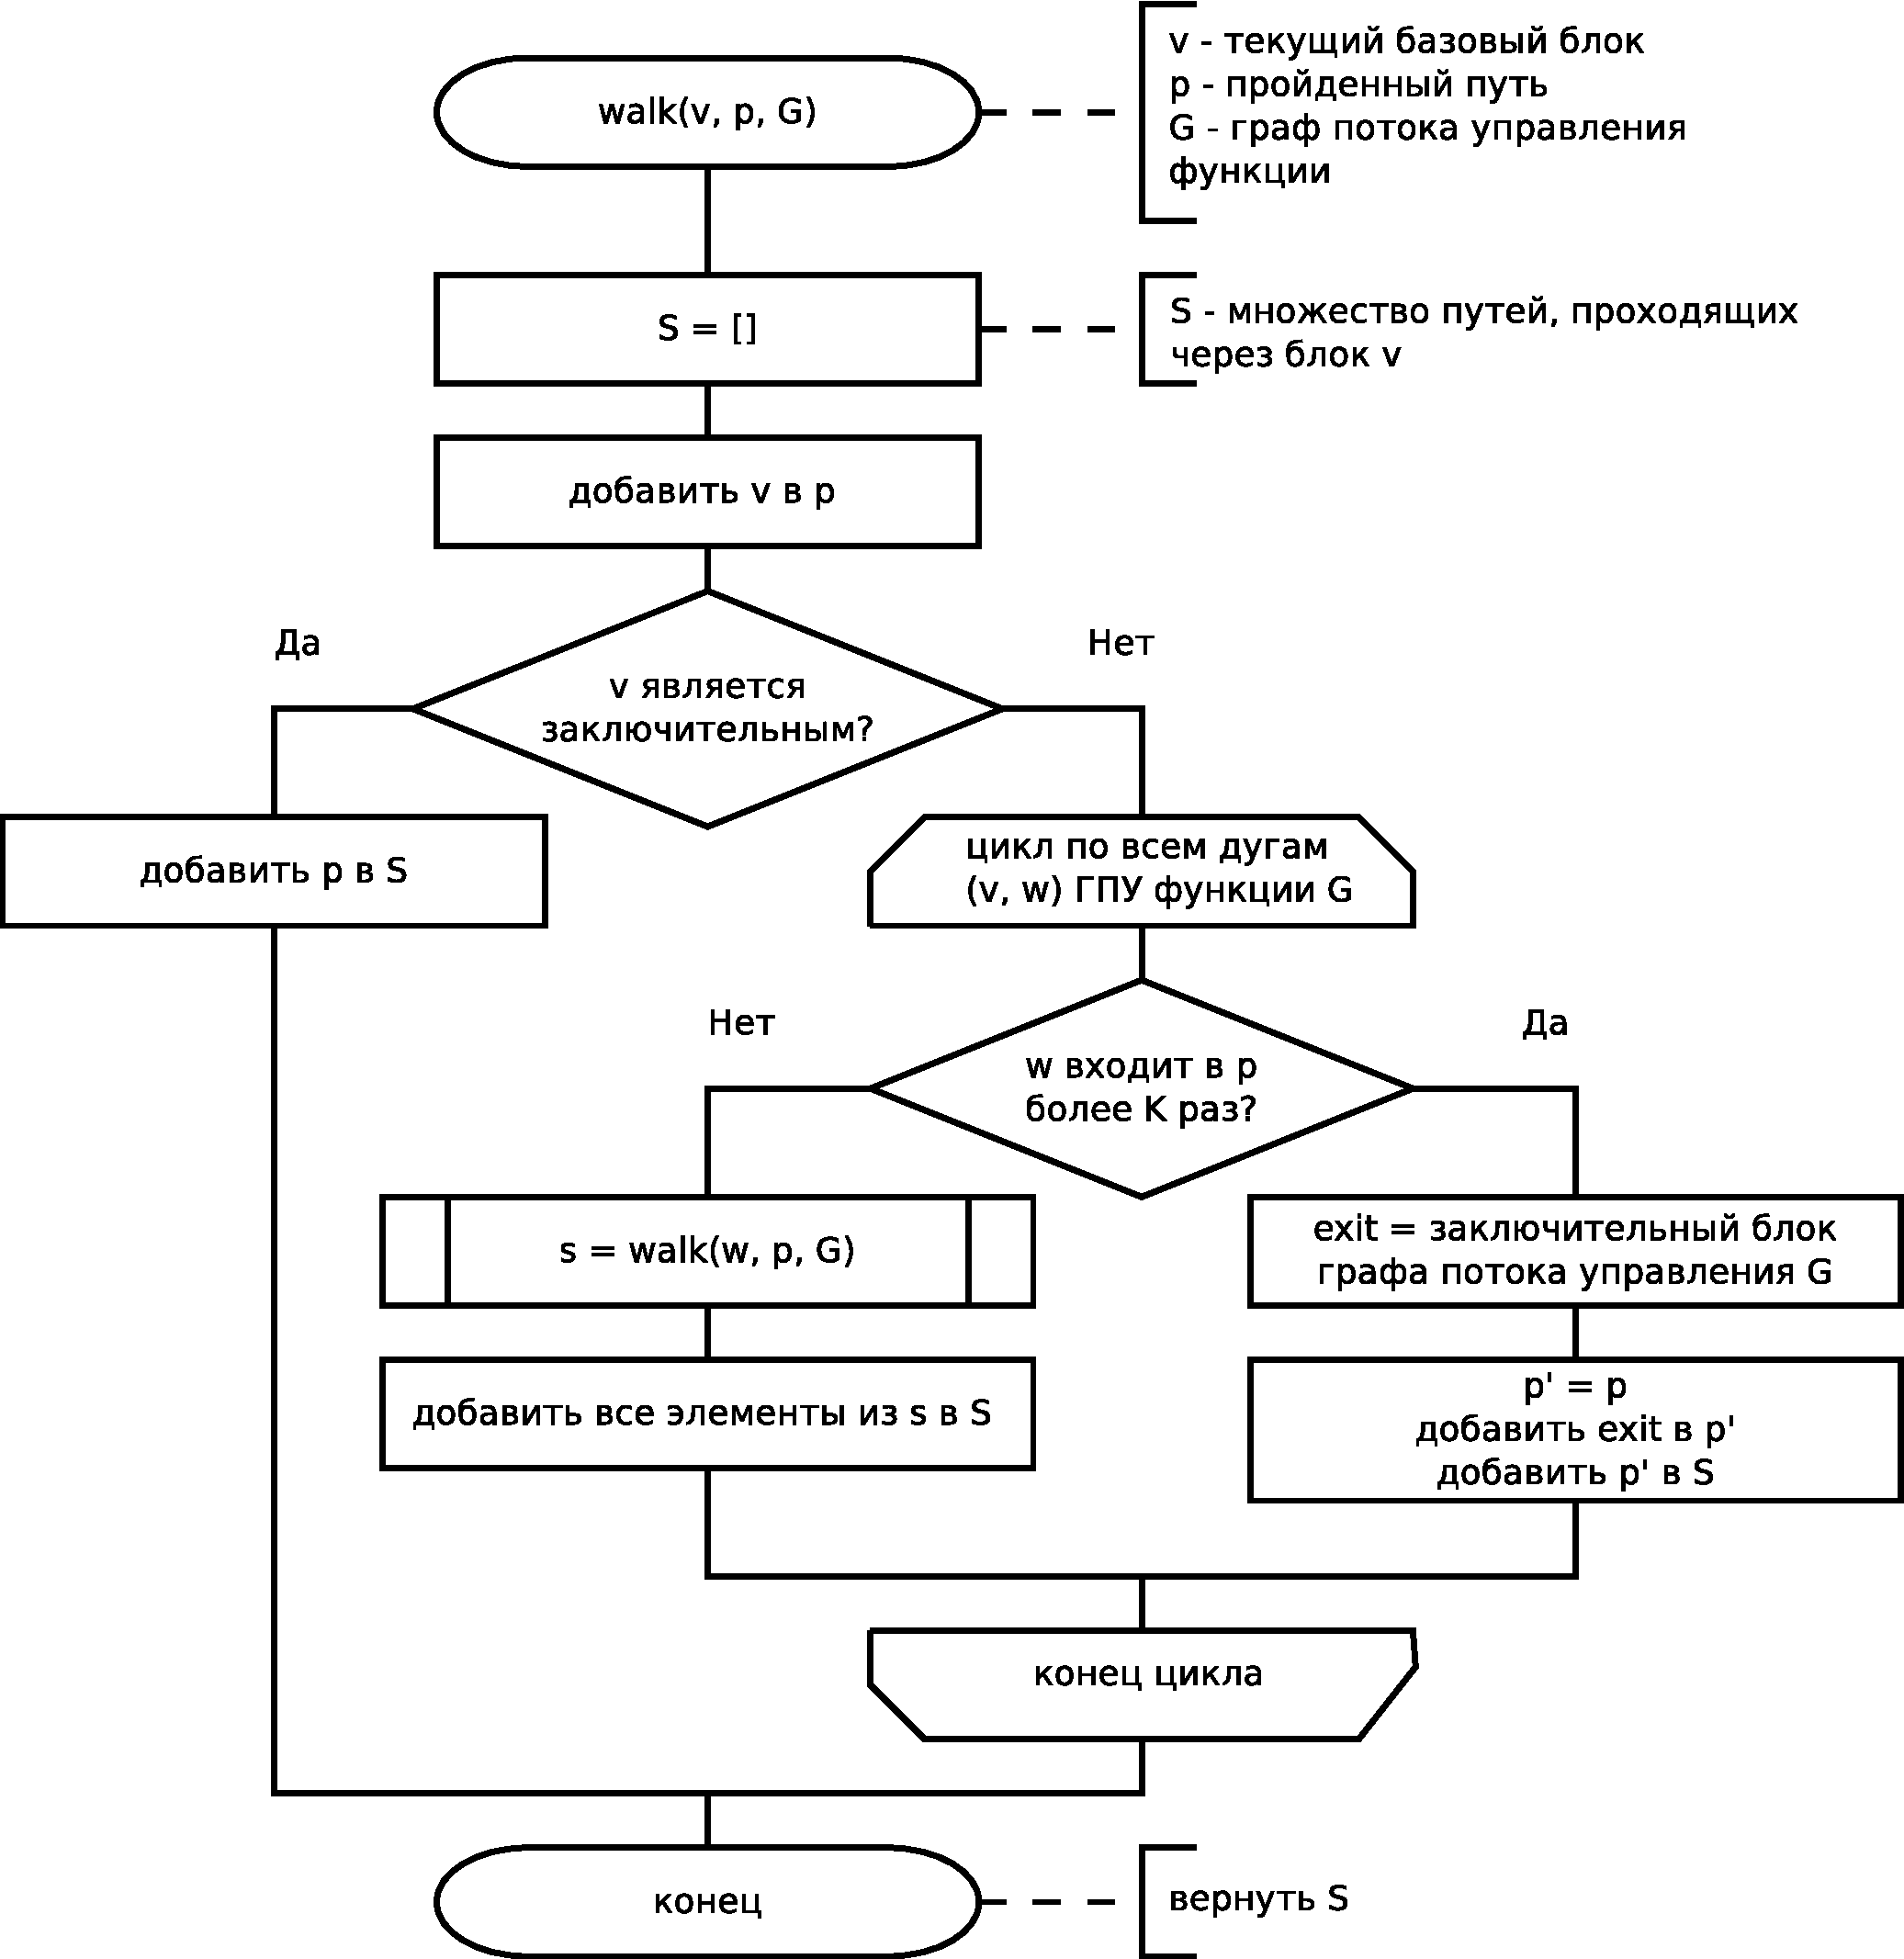
\includegraphics[width=\textwidth]{inc/dia/build-pathes}
  \caption{Схема алгоритма построения множества анализируемых путей выполнения функции}
  \label{fig:build-pathes}
\end{figure}
 
\section{Построение таблицы защищенного доступа для потоков}

Построение таблиц защищённого доступа для потоков состоит из 5 этапов:

\begin{itemize}
  \item определение состояния перекрестных ссылок для всех инструкций путей,
  \item определения отсносительных множеств блокировок для всех инструкций путей,
  \item определение обобщения относительного множества блокировок для функций,
  \item построение таблиц защищенного доступа для функций,
  \item конкретизация таблиц защищённого доступа для всех точек входа в потоки.
\end{itemize}

Сначала выполняется символьное исполнение каждого из путей для определения изменения состояний перекрестных ссылок во время выполнения каждого пути. Затем на основе этого выполняется вычисление относительных множеств блокировок для каждой инструкции на каждом из путей. После анализа всех путей выполнения какой-либо функции для неё строится обобщение относительного множества блокировок, которое используется при анализе других  функций, в которых производится её вызов. На основе путей, размеченных состояниями перекрёстных ссылок и относительными множествами блокировок, строятся таблицы защищенного доступа для всех функций. После чего ищутся все места создания потоков.  Для каждого из них на основе имеющихся таблиц защищенного доступа для функций и известных состояний перекрестных ссылок на момент создания производится конкретизация уже имеющихся таблиц для функций с учётом передаваемых при инициализации потоков значений. Схема построения таблиц защищённого доступа для потоков представлена на рис.~\ref{fig:form-tables}. Рассмотрим далее каждый из представленных этапов подробнее.

\begin{figure}
  \centering
  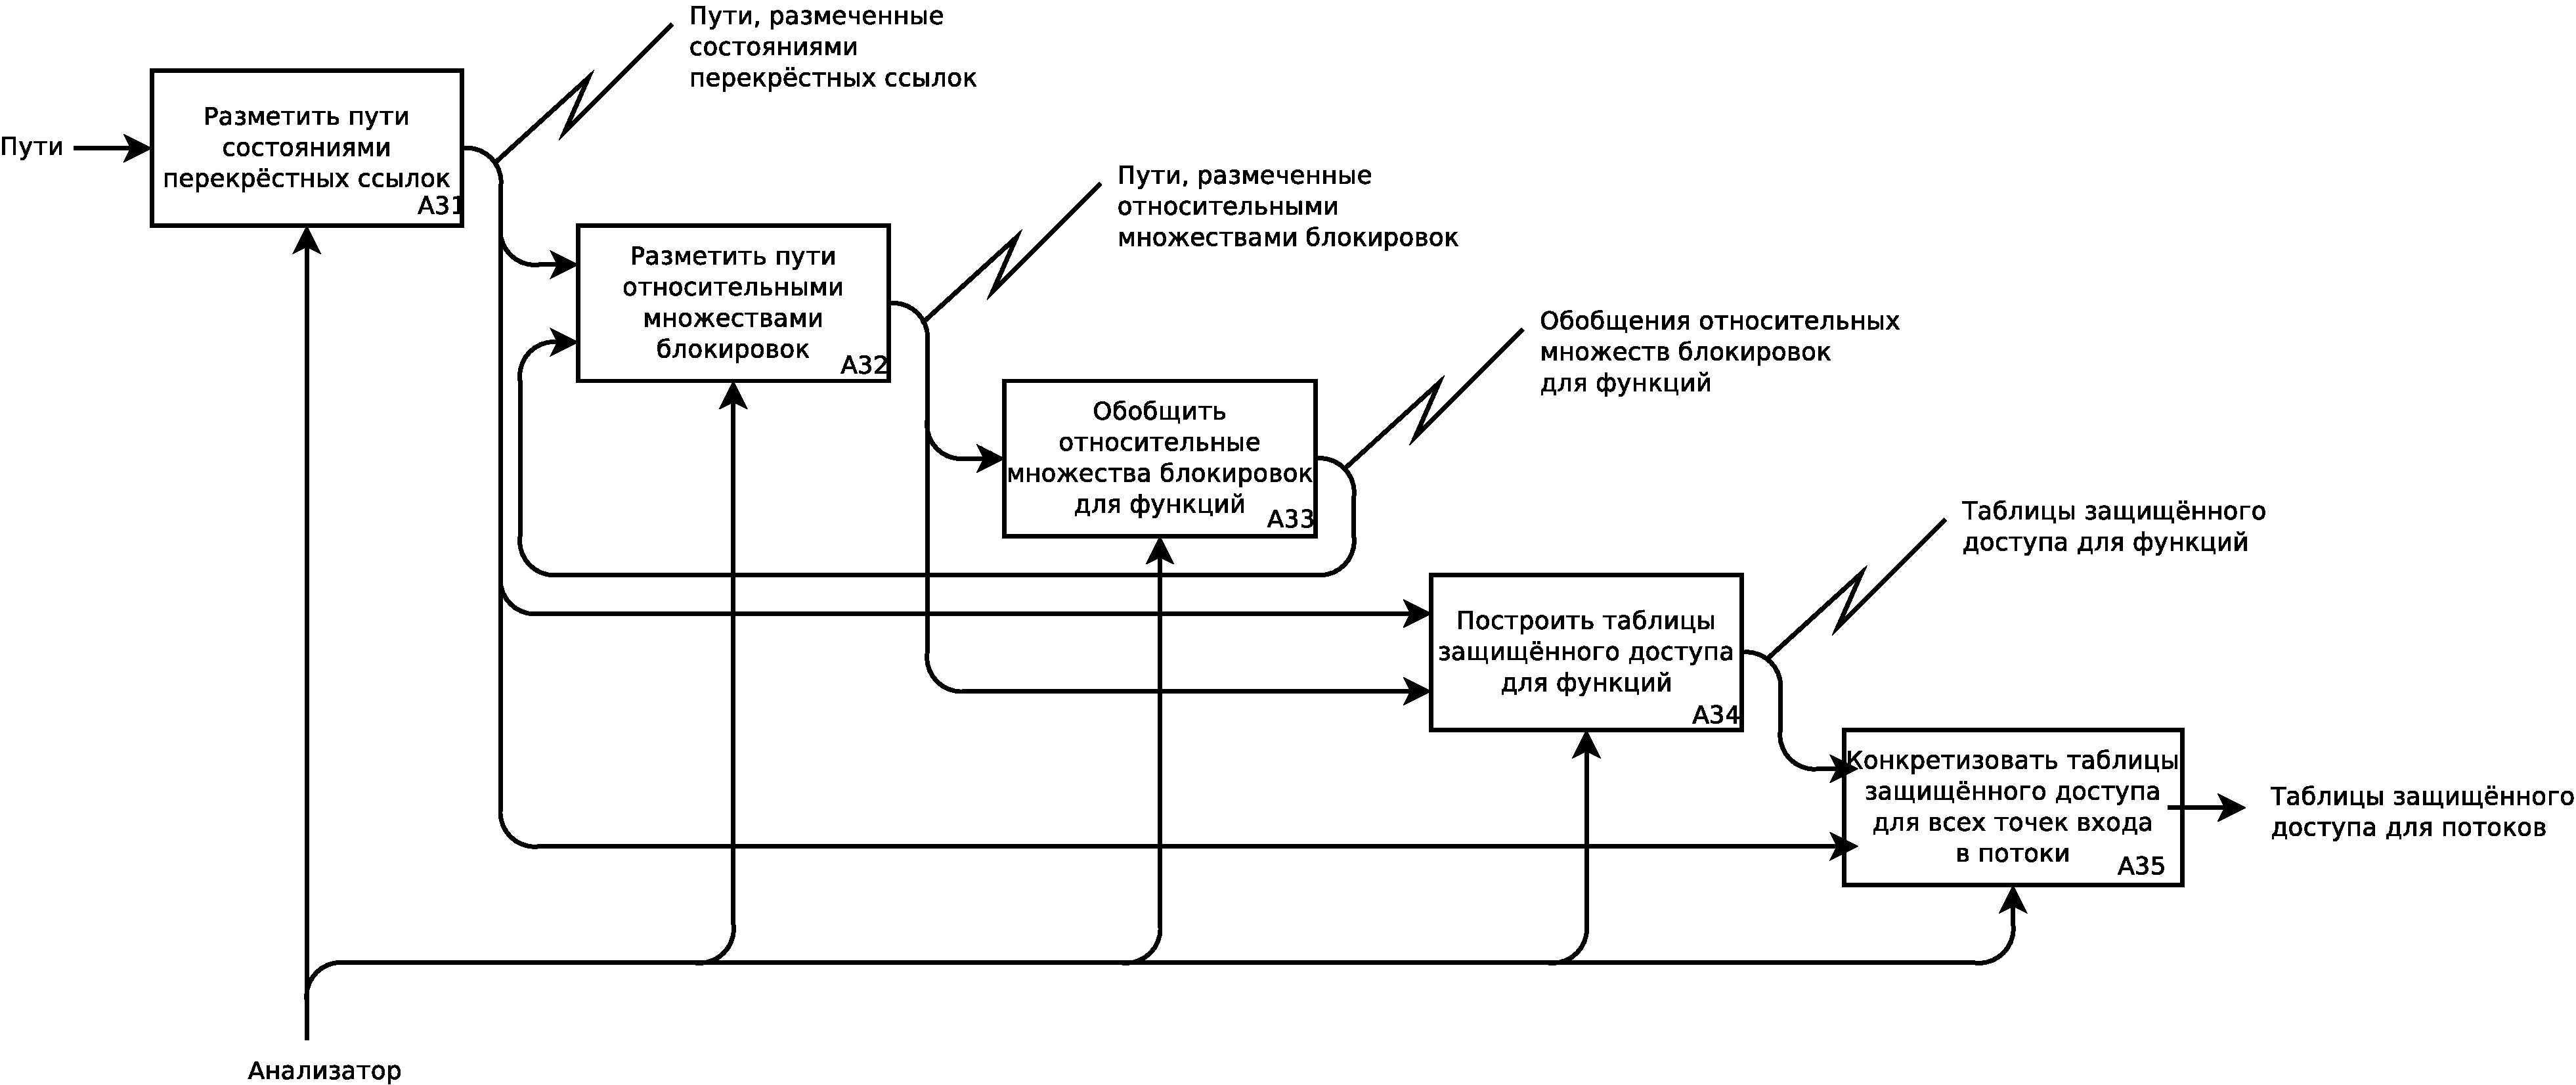
\includegraphics[width=\textwidth]{inc/dia/form-tables}
  \caption{Схема построения таблиц защищенного доступа для потоков}
  \label{fig:form-tables}
\end{figure}

\section{Определение состояния перекрёстных ссылок}

Для определения состояния перекрёстных ссылок для каждой инструкции на каждом анализируемом пути используется символьное исполнение. Анализируемые инструкции присваивания, производимые действия и примеры приведены в таблице~\ref{tab:assignment}.

\begin{center}
  \begin{longtable}{|p{0.20\textwidth}|p{0.40\textwidth}|p{0.40\textwidth}|}
    \caption{Анализируемые инструкции присваивания}
    \label{tab:assignment}
    \\ \hline
    \textbf{Инструкция} & \textbf{Действия} & \textbf{Пример} \\
    \hline \endfirsthead
    \subcaption{Продолжение таблицы~\ref{tab:assignment}}
    \\ \hline \endhead
    \hline \subcaption{Продолжение на след. стр.}
    \endfoot
    \hline \endlastfoot
    $p=q$ & Пусть переменная $q$ из правой части оператора присваивания ссылается на некоторую переменную $a$. Тогда после выполнения оператора присваивания переменная $p$ из левой части оператора присваивания будет сссылаться на переменную $a$. & \raisebox{-\totalheight}{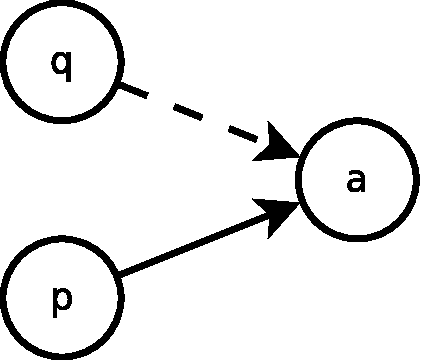
\includegraphics[scale=0.5]{inc/dia/aliases1}}\\
    \hline
    $p=\&q$ & После выполнения оператора присваивания переменная $p$ из левой части оператора присваивания будет ссылаться на переменую $q$ из правой части оператора присваивания. & \raisebox{-\totalheight}{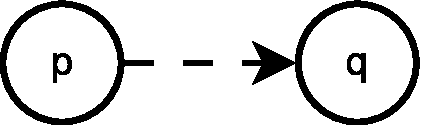
\includegraphics[scale=0.5]{inc/dia/aliases2}} \\
    \hline
    $p=*q$ & Пусть $a$ - переменная, на которую ссылается переменная $q$ из правой части оператора присваивания, $b$ - переменная, на которую ссылается переменная $a$. Тогда после выполнения инструкции присваивания переменная $p$ из левой части оператора присваивания будет ссылаеться на переменную $a$.  & \raisebox{-\totalheight}{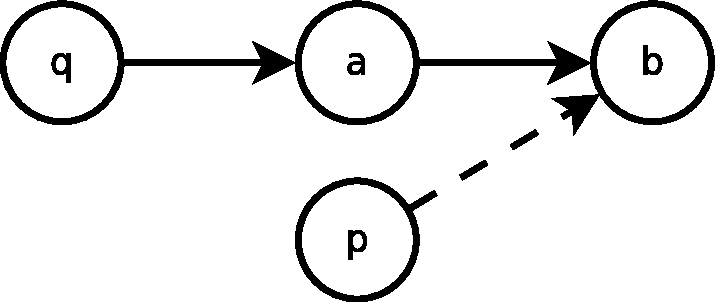
\includegraphics[scale=0.5]{inc/dia/aliases3}} \\
    \hline
    $*p=q$ & Пусть $a$ - переменная, на которую ссылается переменная $q$ из правой части оператора присваивания, $b$ - переменная, на которую ссылается переменная $p$ из левой части оператора присваивания. Тогда после выполнения инструкции присваивания переменная $b$ будет ссылаться на переменную $a$. & \raisebox{-\totalheight}{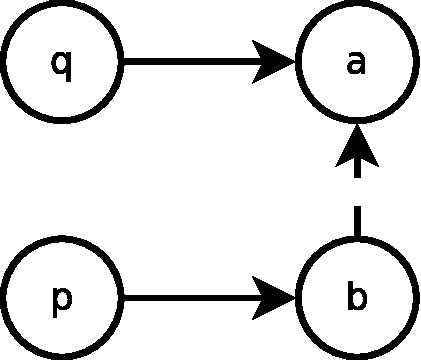
\includegraphics[scale=0.5]{inc/dia/aliases4}} \\
    \hline
    $*p=\&q$ & Пусть переменная $p$ из левой части оператора присваивания ссылается на переменную $a$. Тогда после выполнения инструкции присваивания переменная $a$ будет ссылатсья на переменную $q$ из правой части оператора присваивания. & \raisebox{-\totalheight}{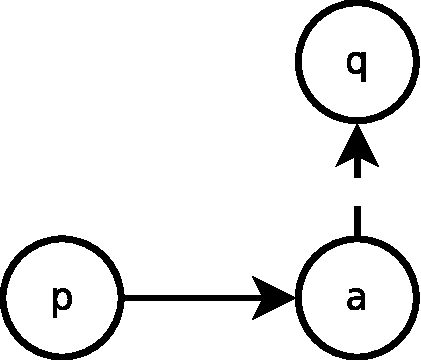
\includegraphics[scale=0.5]{inc/dia/aliases5}} \\
    \hline
    $*p=*q$ & Пусть переменная $q$ из правой части оператора присваивания ссылается на переменную $a$, переменная $a$ ссылается на переменную $b$ и переменная $p$ из левой части оператора присваивания ссылается на переменную $c$. Тогда после выполнения инструкции присваивания переменная $c$ будет ссылаться на переменную $b$. & \raisebox{-\totalheight}{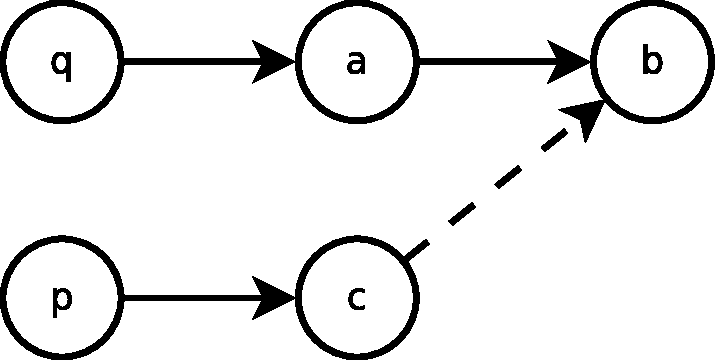
\includegraphics[scale=0.5]{inc/dia/aliases6}} \\
  \end{longtable}
\end{center}

\section{Вычисление относительного множества блокировок и его обобщения}

Под относительным множеством блокировок $L$ будем понимать пару $(L_{+}, L_{-})$, состоящую из множества захваченных блокировок $L_{+}$ и множества освобожденных блокировок $L_{-}$. Оно отражает изменение множества захваченных блокировок, производимое во время некоторого пути выполнения функции.

Перед началом анализа каждого пути выполнения функции относительное множество блокировок полагается пустым. Далее производится последовательный анализ инструкций, встречаемых в пути. Изменение относительного множества блокировок может быть выполнено только в момент вызова какой-либо функции. Для получения измененного относительного множества блокировок после вызова функции используется функция $lock\_update((L_{+}, L_{-}), (L_{+}', L_{-}')) = ((L_{+} \cup L_{+}') - L_{-}', (L_{-} \cup L_{-}') - L_{+}')$. Её первым аргументом является текущее относительное множество блокировок, полученное к моменту вызова функции, а вторым - обобщение относительного множества блокировок вызываемой функции, в котором вхождения формальных параметров функции заменяются на соответствующие им передаваемые при вызове аргументы. Схема алгоритма вычисления относительного множества блокировок при анализе пути выполнения функции представлена на рис.~\ref{fig:build-relative-lockset}.

\begin{figure}
  \centering
  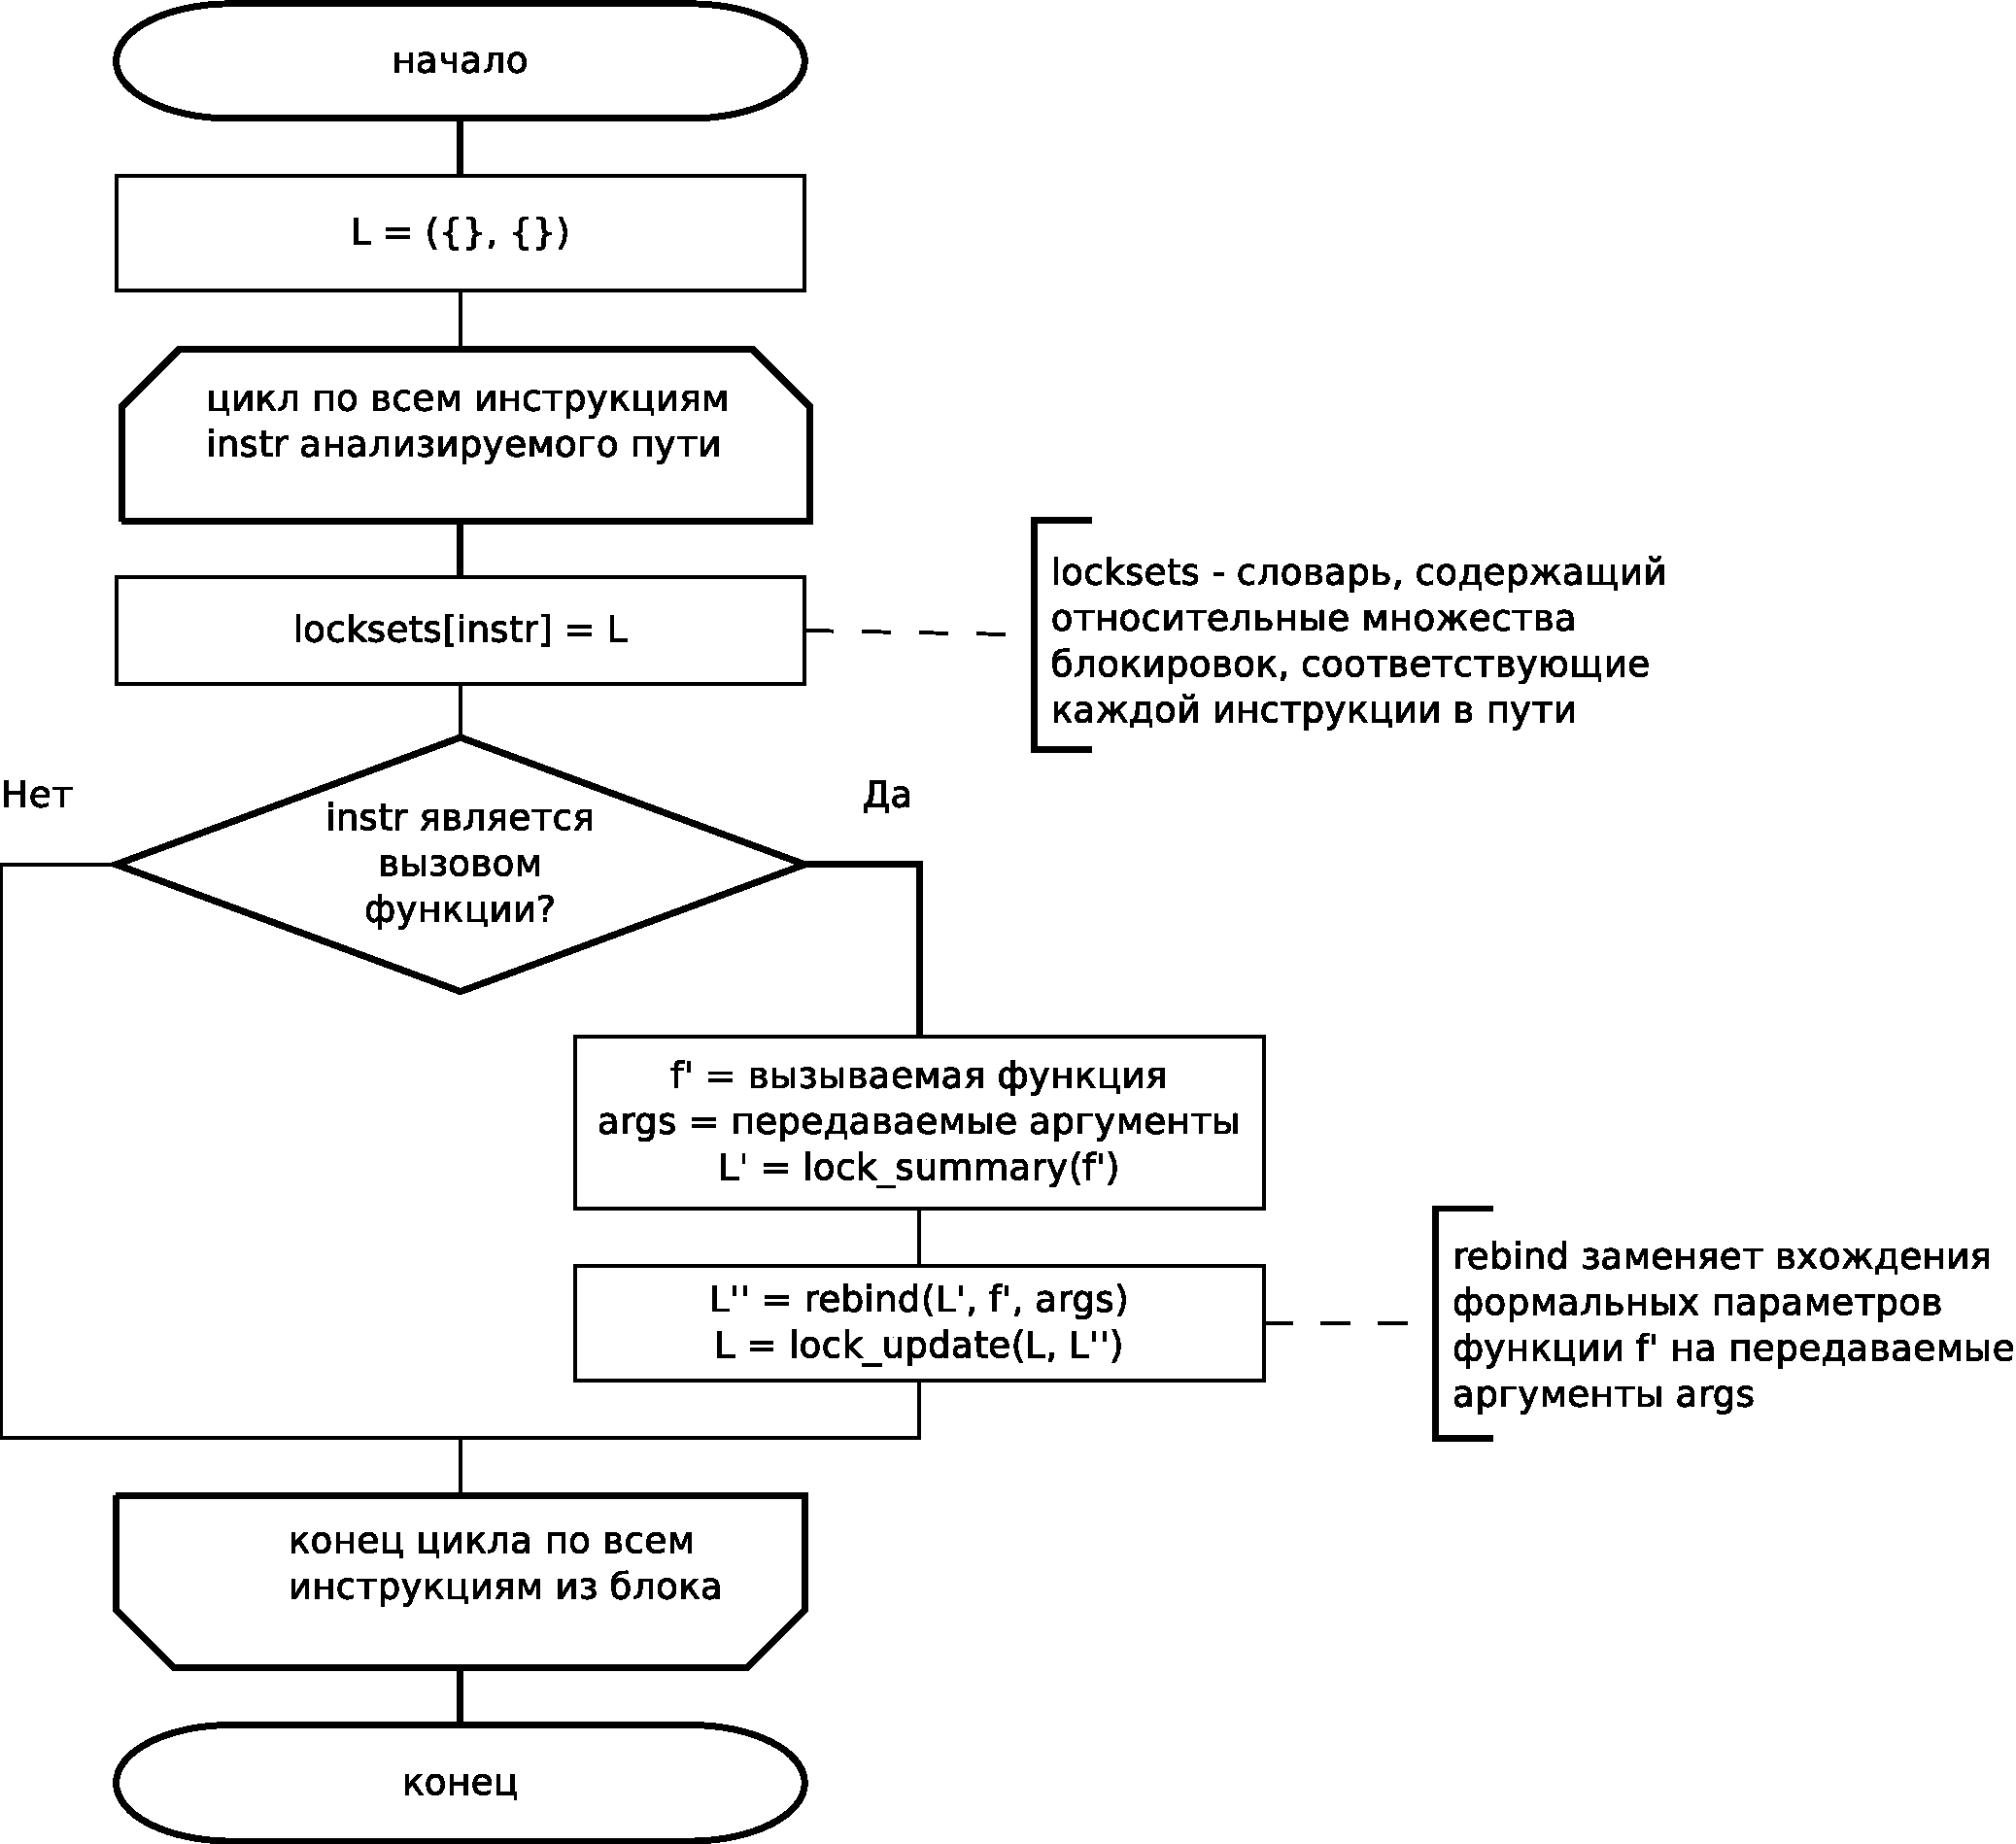
\includegraphics[width=\textwidth]{inc/dia/build-relative-lockset}
  \caption{Схема алгоритма вычисления относительного множества блокировок при анализе пути}
  \label{fig:build-relative-lockset}
\end{figure}

Под обобщением относительного множества блокировок $lock\_summary(f)$ для некоторой функции $f$ понимается относительное множество блокировок, отражающее изменение состояния множества захваченных блокировок во время выполнения функции вне зависимости от выбранного пути выполнения. Для его вычисления необходимо сначала определить относительные множества блокировок, получаемые в конце каждого из анализируемых путей выполнения функции. После чего множество освобожденных блокировок в обобщении будет вычислено как объединение всех множеств освобожденных блокировок, полученных в конце выполнения каждого из анализируемых путей функции, а множество захваченных - как пресечение полученных множеств захваченных блокировок для каждого из путей за вычетом уже подсчитанного множества освобожденных блокировок из обобщения. Таким образом обобщение относительного множества блокировок для функции будет иметь вид $lock\_summary(f) = ((\bigcup_{i \in N}L_{+}[i])/(\bigcap_{i \in N}L_{-}[i]), (\bigcup_{i \in N}L_{-}[i]))$, где $N$ - количество анализируемых путей исполнения функции, а $L_{+}[i]$ и $L_{-}[i]$ - множества захваченных и освобожденных блокировок, полученные на $i$-м анализируемом пути соответственно.

Для функций захвата и освобождения блокировок обобщения заранее известны, и их не требуется вычислять. Так для функции захвата некоторой блокировки $l_{a}$ обобщение относительного множества блокировок будет равным $(\{l_{a}\}, \{\})$, а для функции освобождения - $(\{\}, \{l_{r}\})$, где $l_{r}$ - освобождаемая блокировка.

\section{Построение таблиц защищенного доступа}
\label{sec:build-tables}

Под защищенным доступом $A$ будем понимать тройку $(o, L, k)$, где $o$ - lvalue \cite{Kernigan}, к которому производится доступ, $L$ - относительное множество блокировок на момент доступа, $k$ - тип доступа (<<чтение>> или <<запись>>). Таблицей защищенного доступа будем называть множество всех защищенных доступов, производимых во всех анализируемых путях выполнения функции.

Вначале анализа функции соответствующая ей таблица защищенного доступа полагается пустой. Затем по мере анализа различных путей исполнения функции в неё добавляются соответствующие защищенные доступы. Для построения данной таблицы производится последовательный анализ инструкций, выполняемых на каждом из путей. Если текущая анализируемая инструкция содержит доступ к разделяемой переменной (области памяти), то в таблицу добавляется соответствующая запись. Под разделяемой областью в контексте анализа функции понимаются глобальные переменнные и формальные параметры функции, являющиеся указателями. В случае, когда анализируемая инструкция является вызовом функции, нужно выполнить конкретизацию соответствующей ей таблицы защищенного доступа, и добавить записи из полученной конкретизованной таблицы в таблицу защищенного доступа анализируемой функции. Схема алгоритма конкретизации представлена на рис.~\ref{fig:udpate-access}. При конкретизации таблицы защищенного доступа сначала выполняется замена всех вхождений формальных параметров функции на соответствующие им передаваемые аргументы. После чего из полученной таблицы выбираются все записи, соответствующие разделяемым областям в контексте вызывающей функции. Затем выполняется модификация относительных множеств блокировок для каждой записи с использованием функции $lock\_update$. Первым аргументом в неё передается множество блокировок полученное до вызова функции, а вторым - относительное множество блокировок из соответствующей записи таблицы.

\begin{figure}
  \centering
  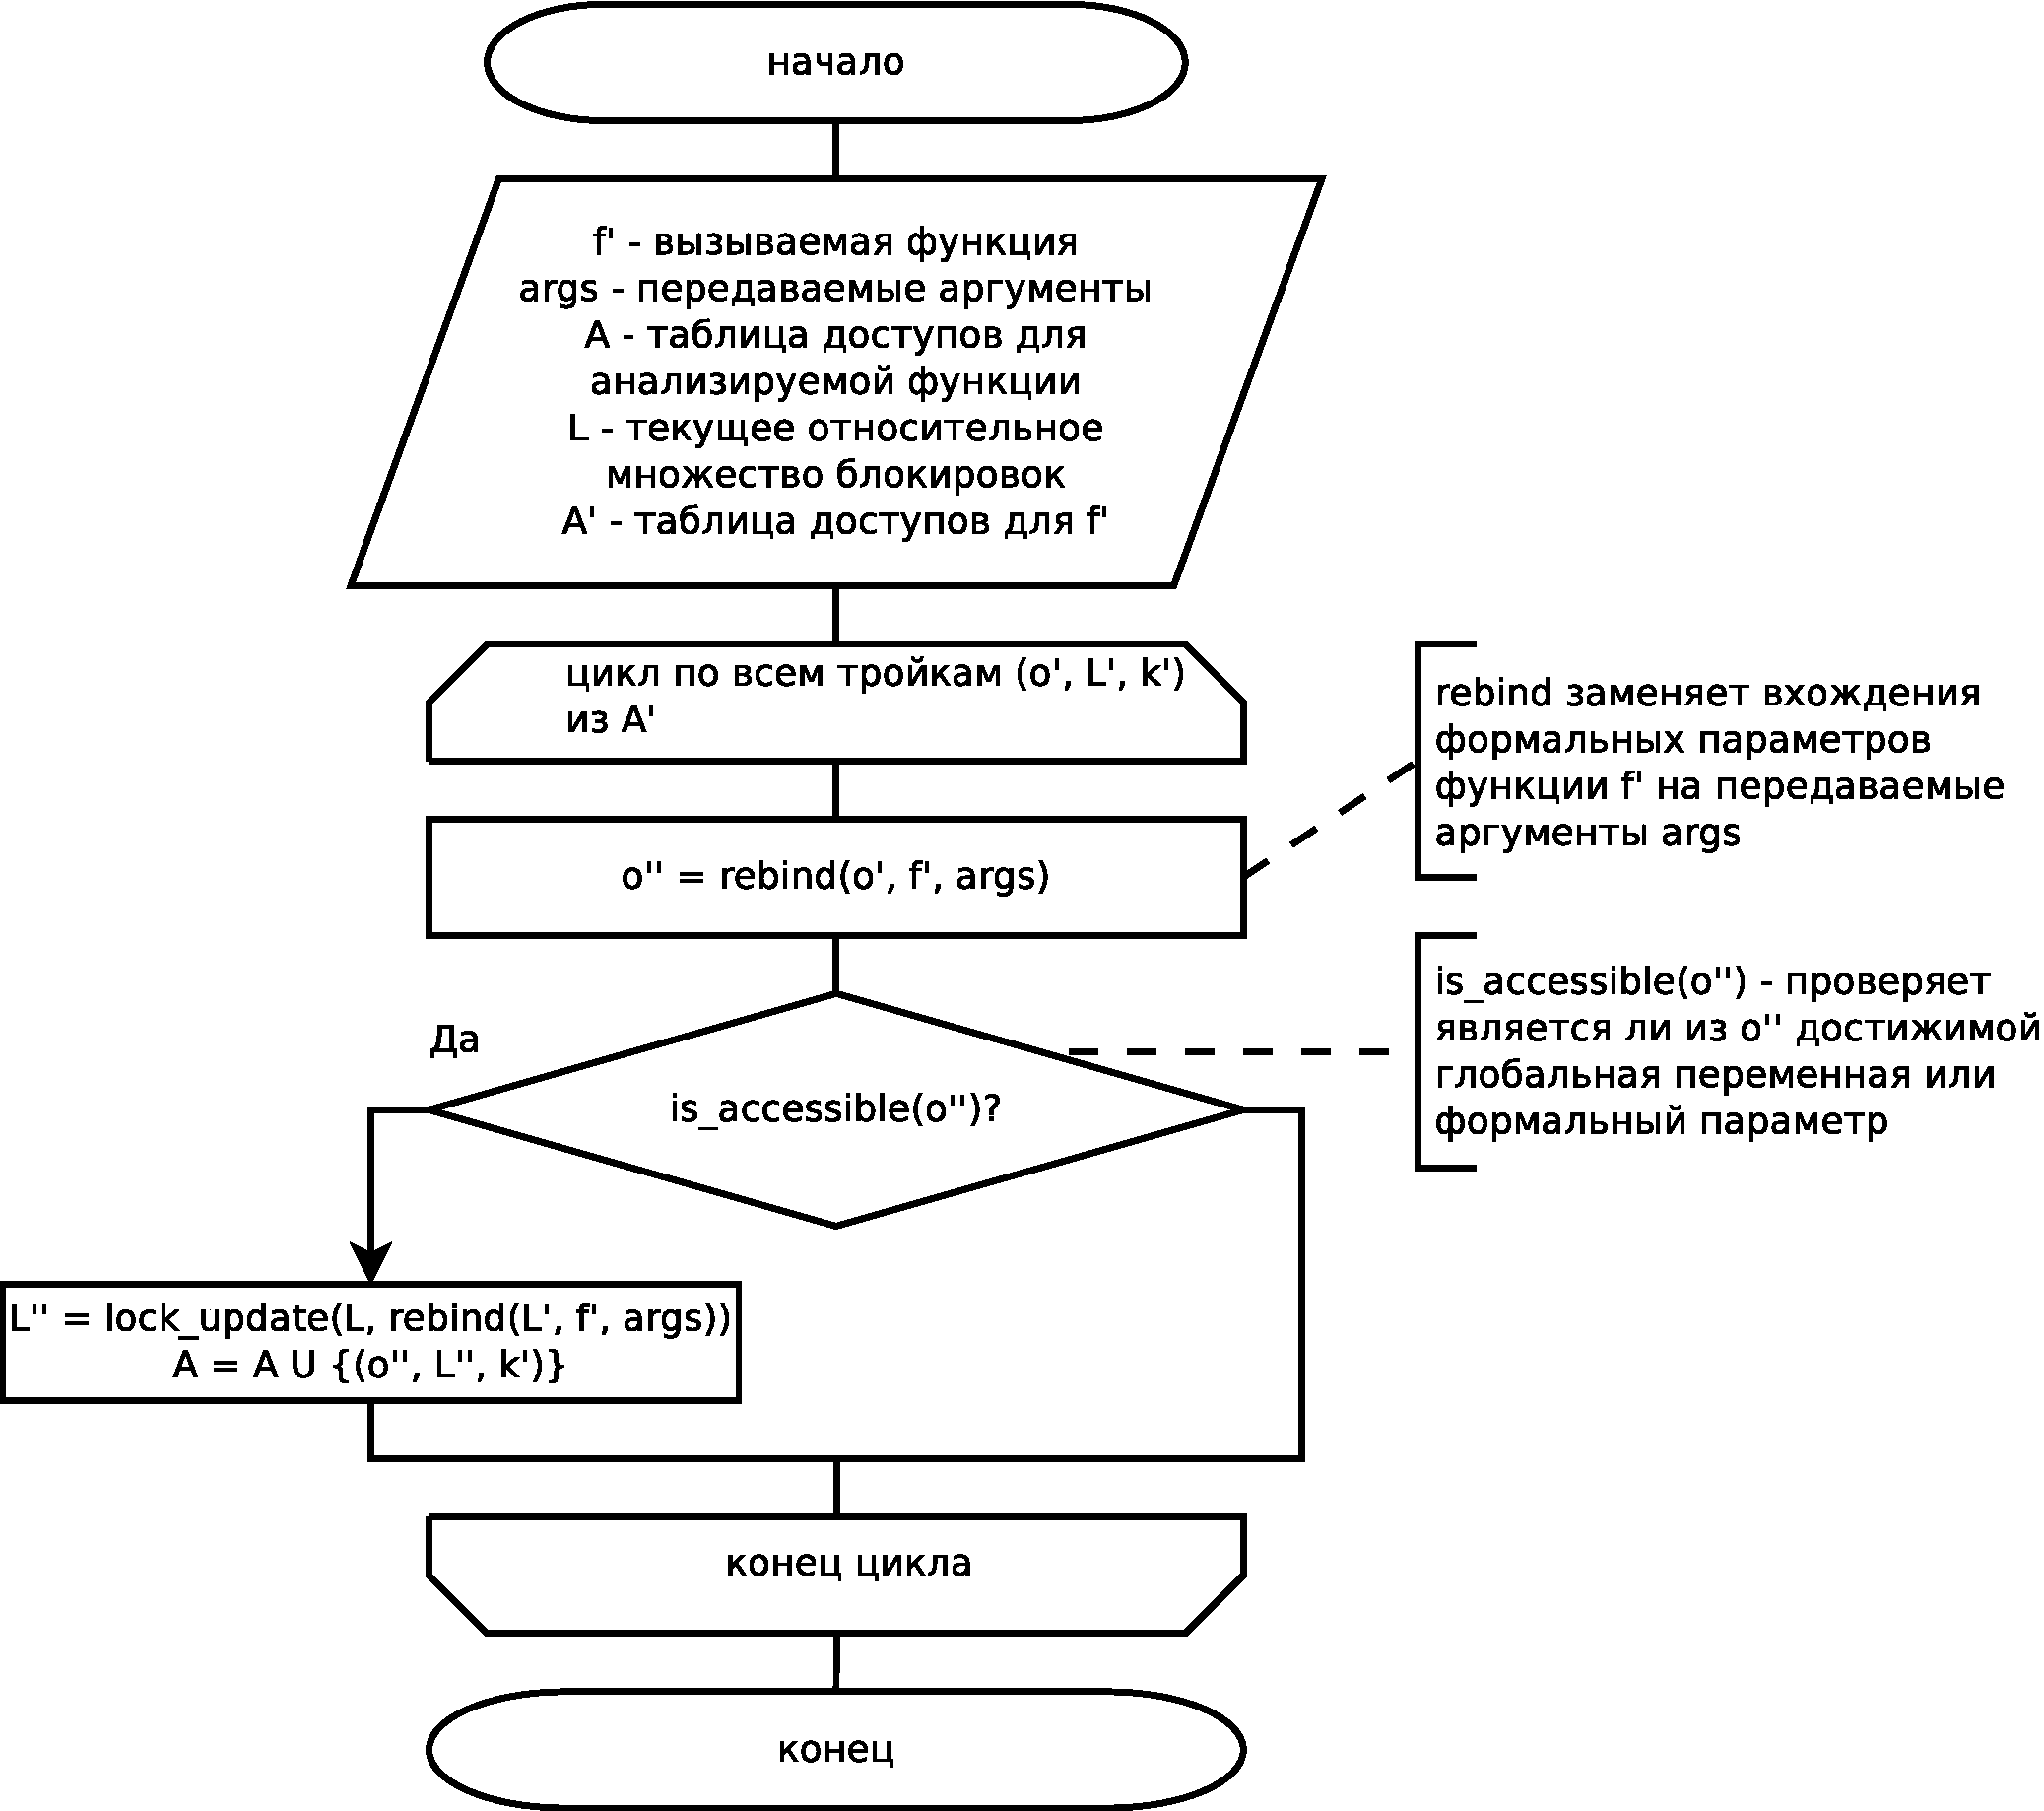
\includegraphics[width=\textwidth]{inc/dia/update-access}
  \caption{Схема алгоритма конкретизации таблицы защищенного доступа функции}
  \label{fig:update-access}
\end{figure}

\section{Определение мест возможного возникновения гонок}

Для определения мест возможного возникновения гонок необходимо предварительно выявить все точки входа в потоки и выполнить конкретизацию соответствующих им таблиц защищенного доступа функций. Алгоритм конкретизации таблиц описан в~\ref
{sec:build-tables}. После конкретизации таблиц для каждой точки входа в поток производится перебор всех пар точек входа в потоки и сравнение соответствующих им таблиц защищённого доступа. В случае, когда в таблицах, соответствующих разным точкам входа, присутствуют доступы к одной и той же области, и при этом хотя бы один из них является доступом на запись, и пересечение множеств захваченных блокировок пусто, то данная область помечается как потенциально опасное место возникновения гонок. Схема алгоритма представлена на рис.~\ref{fig:generate-warnings}.

\begin{figure}
  \centering
  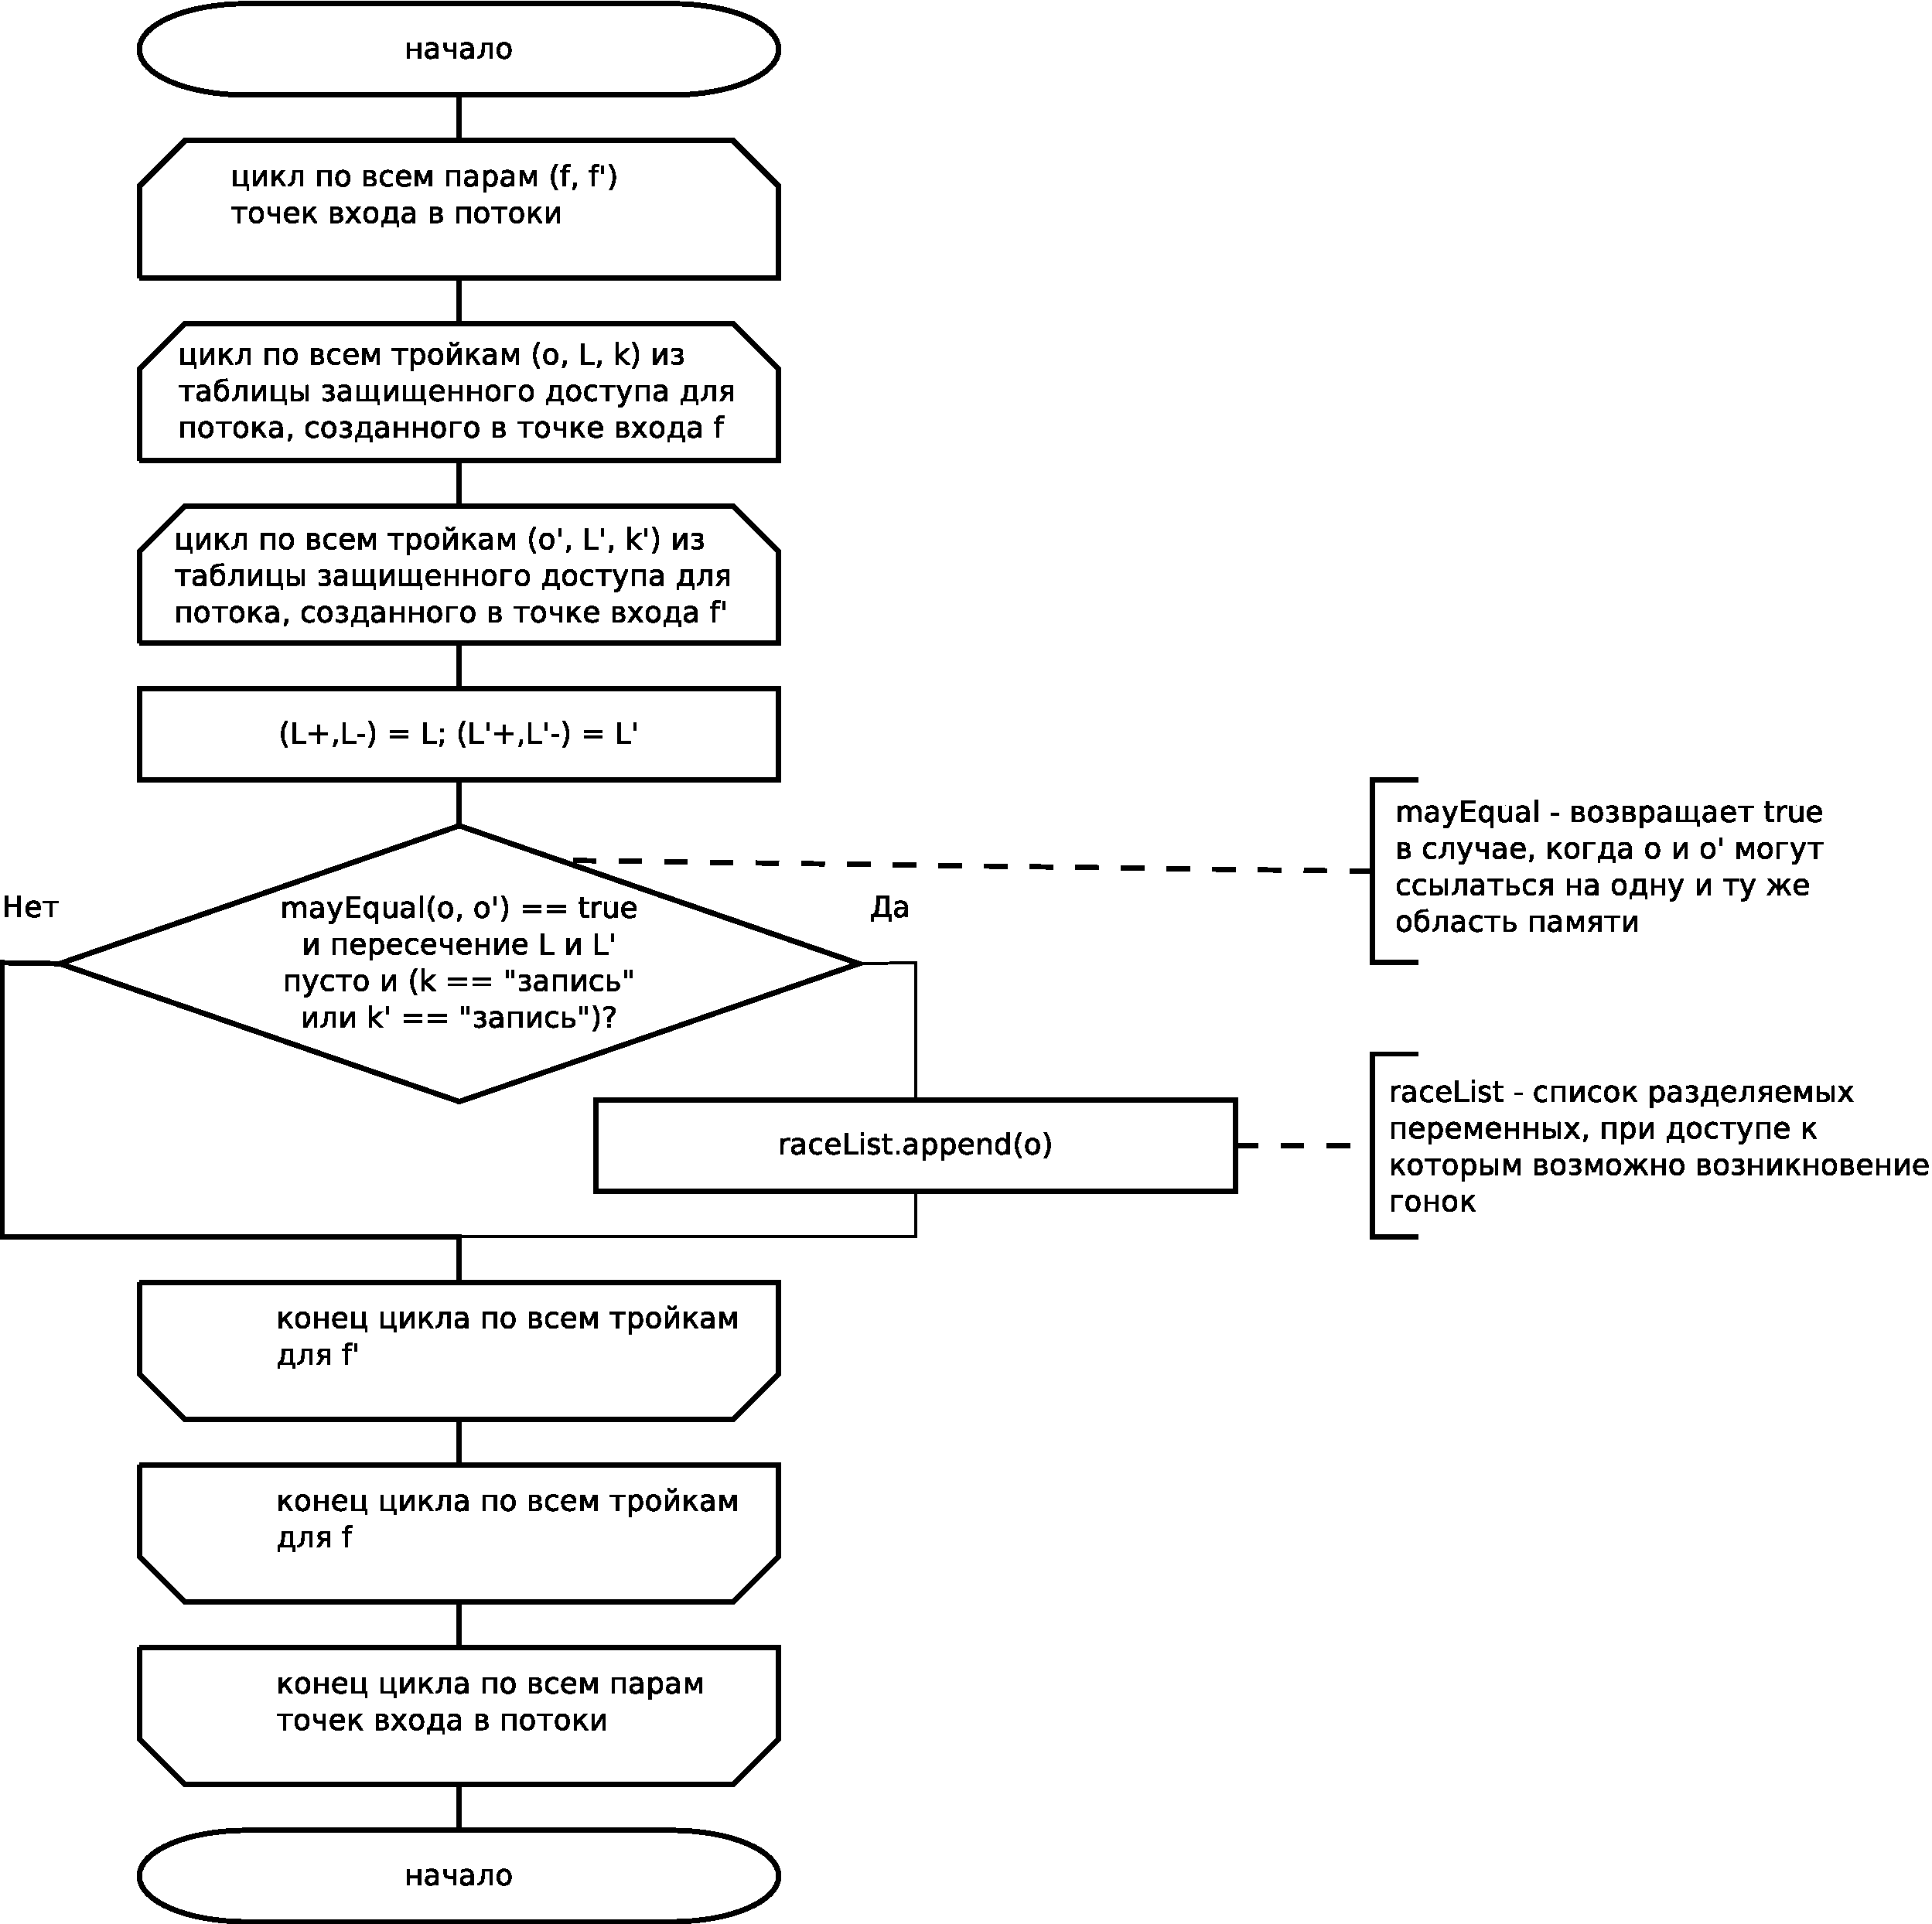
\includegraphics[width=\textwidth]{inc/dia/generate-warnings}
  \caption{Схема алгоритма определения мест возможного возникновения гонок}
  \label{fig:generate-warnings}
\end{figure}

\section{Выводы}

Разработан метод статического поиске гонок на основе относительного множества блокировок. Описаны алгоритмы, применяемые на каждом из этапов метода. Представлены ограничения, накладываемые на анализируемые программы.
